% Build from docs/: make 2026_10_09_interferer_hunt.tex
% Figures are tracked copies in docs/images/interferer_hunt/ of the bench
% outputs beneath build/; the one-off scripts that made them sit beside them, and
% the code-spectrum figures are regenerated by
% uv run python -m flow.analysis.runner adc_interferer_study.
% Shared FRIDA Beamer style. Start each slide deck with % Shared FRIDA Beamer style. Start each slide deck with % Shared FRIDA Beamer style. Start each slide deck with \input{style.tex}.
\documentclass[aspectratio=169,compress]{beamer}
\usepackage[T1]{fontenc}
\usepackage{lmodern,graphicx,xcolor,amsmath,booktabs,array,tikz,listings,etoolbox}

% Decks are built from docs/slides; figures live beside docs and in docs/images.
\graphicspath{{../}{./}}

\definecolor{NordBody}{HTML}{4C566A}
\definecolor{NordBlue}{HTML}{5E81AC}
\definecolor{NordRed}{HTML}{BF616A}
\definecolor{NordGreen}{HTML}{A3BE8C}
\definecolor{NordOrange}{HTML}{D08770}
\definecolor{NordPurple}{HTML}{B48EAD}
\definecolor{NordPanel}{HTML}{ECEFF4}

\newcommand{\framesource}{}
\BeforeBeginEnvironment{frame}{\gdef\framesource{}}
\newcommand{\slidesource}[1]{\gdef\framesource{#1}}
\setbeamertemplate{footline}{%
  \hbox{%
    \begin{beamercolorbox}[wd=.12\paperwidth,ht=2.7ex,dp=1.2ex,leftskip=1em]{page number in head/foot}%
      \usebeamerfont{page number in head/foot}\insertframenumber\,/\,\inserttotalframenumber
    \end{beamercolorbox}%
    \begin{beamercolorbox}[wd=.88\paperwidth,ht=2.7ex,dp=1.2ex,right,rightskip=1em]{normal text}%
      \fontsize{5.5}{6.5}\selectfont\ifx\framesource\empty\else Sources:\enspace\framesource\fi
    \end{beamercolorbox}%
  }%
}
\beamertemplatenavigationsymbolsempty
\setbeameroption{hide notes}

% Opt in for decks with sections; shorter decks keep the full frame height.
\newcommand{\slideprogressnavigation}{%
  \useoutertheme[subsection=false]{miniframes}
  \setbeamercolor{section in head/foot}{fg=NordBlue,bg=white}
  \setbeamercolor{mini frame}{fg=NordBlue,bg=white}
  \setbeamercolor{lower separation line head}{bg=NordPanel}
  \setbeamerfont{section in head/foot}{size=\tiny}

  \newif\ifnavbeforecurrent
  \pretocmd\insertnavigation{\navbeforecurrenttrue}{}{}

  \newcommand{\fridanavigationdot}{%
    \begin{pgfpicture}{0pt}{0pt}{0.1cm}{0.1cm}
      \pgfpathcircle{\pgfpoint{0.05cm}{0.05cm}}{0.05cm}
      \ifnavbeforecurrent
        \pgfusepath{fill,stroke}
      \else
        \pgfusepath{stroke}
      \fi
    \end{pgfpicture}%
  }

  \defbeamertemplate*{mini frame}{frida progress}{%
    \begin{pgfpicture}{0pt}{0pt}{0.1cm}{0.1cm}
      \pgfpathcircle{\pgfpoint{0.05cm}{0.05cm}}{0.05cm}
      \pgfusepath{fill,stroke}
    \end{pgfpicture}%
    \global\navbeforecurrentfalse
  }
  \defbeamertemplate*{mini frame in current section}{frida progress}{\fridanavigationdot}
  \defbeamertemplate*{mini frame in current subsection}{frida progress}{\fridanavigationdot}
  \defbeamertemplate*{mini frame in other section}{frida progress}{\fridanavigationdot}
  \defbeamertemplate*{mini frame in other subsection}{frida progress}{\fridanavigationdot}
  \setbeamertemplate{mini frame}[frida progress]
  \setbeamertemplate{mini frame in current section}[frida progress]
  \setbeamertemplate{mini frame in current subsection}[frida progress]
  \setbeamertemplate{mini frame in other section}[frida progress]
  \setbeamertemplate{mini frame in other subsection}[frida progress]
}

\setbeamerfont{frametitle}{size=\large}
\setbeamerfont{framesubtitle}{size=\small}
\setbeamercolor{normal text}{fg=NordBody}
\setbeamercolor{title}{fg=NordBlue}
\setbeamercolor{frametitle}{fg=NordBlue}
\setbeamercolor{framesubtitle}{fg=NordBody}
\setbeamercolor{structure}{fg=NordBlue}
\setbeamercolor{itemize/enumerate body}{fg=NordBody}
\setbeamercolor{itemize/enumerate subbody}{fg=NordBody}
\setbeamercolor{itemize/enumerate subsubbody}{fg=NordBody}
\setbeamercolor{itemize item}{fg=NordBlue}
\setbeamercolor{itemize subitem}{fg=NordBlue}
\setbeamercolor{itemize subsubitem}{fg=NordBlue}
\setbeamercolor{enumerate item}{fg=NordBlue}
\setbeamercolor{enumerate subitem}{fg=NordBlue}
\setbeamercolor{enumerate subsubitem}{fg=NordBlue}
\setbeamercolor{block title}{fg=NordBlue,bg=NordPanel}
\setbeamercolor{block body}{fg=NordBody,bg=NordPanel!55}
\hypersetup{colorlinks=true,allcolors=NordBlue}

\lstset{%
  basicstyle=\ttfamily\tiny,
  keywordstyle=\color{NordBlue}\bfseries,
  commentstyle=\color{NordBody}\itshape,
  stringstyle=\color{NordOrange},
  showstringspaces=false,
  breaklines=true,
  frame=single,
  backgroundcolor=\color{NordPanel!55},
  rulecolor=\color{NordBody!50},
  xleftmargin=2pt,
  xrightmargin=2pt,
  aboveskip=4pt,
  belowskip=4pt,
}

\newcommand{\placeholder}[2]{%
  \begin{tikzpicture}
    \node[minimum width=#1,minimum height=#2,draw=NordBlue!60,rounded corners=2pt,fill=NordPanel,align=center,text=NordBody]
      {Placeholder\\[-1pt]\scriptsize image not yet available};
  \end{tikzpicture}%
}
\newcommand{\maybeimage}[2][]{%
  \IfFileExists{#2}{\includegraphics[#1]{#2}}{%
    \IfFileExists{../#2}{\includegraphics[#1]{#2}}{\placeholder{0.95\linewidth}{0.30\textheight}}%
  }%
}

\author{Kennedy Caisley}
\institute{University of Bonn}
.
\documentclass[aspectratio=169,compress]{beamer}
\usepackage[T1]{fontenc}
\usepackage{lmodern,graphicx,xcolor,amsmath,booktabs,array,tikz,listings,etoolbox}

% Decks are built from docs/slides; figures live beside docs and in docs/images.
\graphicspath{{../}{./}}

\definecolor{NordBody}{HTML}{4C566A}
\definecolor{NordBlue}{HTML}{5E81AC}
\definecolor{NordRed}{HTML}{BF616A}
\definecolor{NordGreen}{HTML}{A3BE8C}
\definecolor{NordOrange}{HTML}{D08770}
\definecolor{NordPurple}{HTML}{B48EAD}
\definecolor{NordPanel}{HTML}{ECEFF4}

\newcommand{\framesource}{}
\BeforeBeginEnvironment{frame}{\gdef\framesource{}}
\newcommand{\slidesource}[1]{\gdef\framesource{#1}}
\setbeamertemplate{footline}{%
  \hbox{%
    \begin{beamercolorbox}[wd=.12\paperwidth,ht=2.7ex,dp=1.2ex,leftskip=1em]{page number in head/foot}%
      \usebeamerfont{page number in head/foot}\insertframenumber\,/\,\inserttotalframenumber
    \end{beamercolorbox}%
    \begin{beamercolorbox}[wd=.88\paperwidth,ht=2.7ex,dp=1.2ex,right,rightskip=1em]{normal text}%
      \fontsize{5.5}{6.5}\selectfont\ifx\framesource\empty\else Sources:\enspace\framesource\fi
    \end{beamercolorbox}%
  }%
}
\beamertemplatenavigationsymbolsempty
\setbeameroption{hide notes}

% Opt in for decks with sections; shorter decks keep the full frame height.
\newcommand{\slideprogressnavigation}{%
  \useoutertheme[subsection=false]{miniframes}
  \setbeamercolor{section in head/foot}{fg=NordBlue,bg=white}
  \setbeamercolor{mini frame}{fg=NordBlue,bg=white}
  \setbeamercolor{lower separation line head}{bg=NordPanel}
  \setbeamerfont{section in head/foot}{size=\tiny}

  \newif\ifnavbeforecurrent
  \pretocmd\insertnavigation{\navbeforecurrenttrue}{}{}

  \newcommand{\fridanavigationdot}{%
    \begin{pgfpicture}{0pt}{0pt}{0.1cm}{0.1cm}
      \pgfpathcircle{\pgfpoint{0.05cm}{0.05cm}}{0.05cm}
      \ifnavbeforecurrent
        \pgfusepath{fill,stroke}
      \else
        \pgfusepath{stroke}
      \fi
    \end{pgfpicture}%
  }

  \defbeamertemplate*{mini frame}{frida progress}{%
    \begin{pgfpicture}{0pt}{0pt}{0.1cm}{0.1cm}
      \pgfpathcircle{\pgfpoint{0.05cm}{0.05cm}}{0.05cm}
      \pgfusepath{fill,stroke}
    \end{pgfpicture}%
    \global\navbeforecurrentfalse
  }
  \defbeamertemplate*{mini frame in current section}{frida progress}{\fridanavigationdot}
  \defbeamertemplate*{mini frame in current subsection}{frida progress}{\fridanavigationdot}
  \defbeamertemplate*{mini frame in other section}{frida progress}{\fridanavigationdot}
  \defbeamertemplate*{mini frame in other subsection}{frida progress}{\fridanavigationdot}
  \setbeamertemplate{mini frame}[frida progress]
  \setbeamertemplate{mini frame in current section}[frida progress]
  \setbeamertemplate{mini frame in current subsection}[frida progress]
  \setbeamertemplate{mini frame in other section}[frida progress]
  \setbeamertemplate{mini frame in other subsection}[frida progress]
}

\setbeamerfont{frametitle}{size=\large}
\setbeamerfont{framesubtitle}{size=\small}
\setbeamercolor{normal text}{fg=NordBody}
\setbeamercolor{title}{fg=NordBlue}
\setbeamercolor{frametitle}{fg=NordBlue}
\setbeamercolor{framesubtitle}{fg=NordBody}
\setbeamercolor{structure}{fg=NordBlue}
\setbeamercolor{itemize/enumerate body}{fg=NordBody}
\setbeamercolor{itemize/enumerate subbody}{fg=NordBody}
\setbeamercolor{itemize/enumerate subsubbody}{fg=NordBody}
\setbeamercolor{itemize item}{fg=NordBlue}
\setbeamercolor{itemize subitem}{fg=NordBlue}
\setbeamercolor{itemize subsubitem}{fg=NordBlue}
\setbeamercolor{enumerate item}{fg=NordBlue}
\setbeamercolor{enumerate subitem}{fg=NordBlue}
\setbeamercolor{enumerate subsubitem}{fg=NordBlue}
\setbeamercolor{block title}{fg=NordBlue,bg=NordPanel}
\setbeamercolor{block body}{fg=NordBody,bg=NordPanel!55}
\hypersetup{colorlinks=true,allcolors=NordBlue}

\lstset{%
  basicstyle=\ttfamily\tiny,
  keywordstyle=\color{NordBlue}\bfseries,
  commentstyle=\color{NordBody}\itshape,
  stringstyle=\color{NordOrange},
  showstringspaces=false,
  breaklines=true,
  frame=single,
  backgroundcolor=\color{NordPanel!55},
  rulecolor=\color{NordBody!50},
  xleftmargin=2pt,
  xrightmargin=2pt,
  aboveskip=4pt,
  belowskip=4pt,
}

\newcommand{\placeholder}[2]{%
  \begin{tikzpicture}
    \node[minimum width=#1,minimum height=#2,draw=NordBlue!60,rounded corners=2pt,fill=NordPanel,align=center,text=NordBody]
      {Placeholder\\[-1pt]\scriptsize image not yet available};
  \end{tikzpicture}%
}
\newcommand{\maybeimage}[2][]{%
  \IfFileExists{#2}{\includegraphics[#1]{#2}}{%
    \IfFileExists{../#2}{\includegraphics[#1]{#2}}{\placeholder{0.95\linewidth}{0.30\textheight}}%
  }%
}

\author{Kennedy Caisley}
\institute{University of Bonn}
.
\documentclass[aspectratio=169,compress]{beamer}
\usepackage[T1]{fontenc}
\usepackage{lmodern,graphicx,xcolor,amsmath,booktabs,array,tikz,listings,etoolbox}

% Decks are built from docs/slides; figures live beside docs and in docs/images.
\graphicspath{{../}{./}}

\definecolor{NordBody}{HTML}{4C566A}
\definecolor{NordBlue}{HTML}{5E81AC}
\definecolor{NordRed}{HTML}{BF616A}
\definecolor{NordGreen}{HTML}{A3BE8C}
\definecolor{NordOrange}{HTML}{D08770}
\definecolor{NordPurple}{HTML}{B48EAD}
\definecolor{NordPanel}{HTML}{ECEFF4}

\newcommand{\framesource}{}
\BeforeBeginEnvironment{frame}{\gdef\framesource{}}
\newcommand{\slidesource}[1]{\gdef\framesource{#1}}
\setbeamertemplate{footline}{%
  \hbox{%
    \begin{beamercolorbox}[wd=.12\paperwidth,ht=2.7ex,dp=1.2ex,leftskip=1em]{page number in head/foot}%
      \usebeamerfont{page number in head/foot}\insertframenumber\,/\,\inserttotalframenumber
    \end{beamercolorbox}%
    \begin{beamercolorbox}[wd=.88\paperwidth,ht=2.7ex,dp=1.2ex,right,rightskip=1em]{normal text}%
      \fontsize{5.5}{6.5}\selectfont\ifx\framesource\empty\else Sources:\enspace\framesource\fi
    \end{beamercolorbox}%
  }%
}
\beamertemplatenavigationsymbolsempty
\setbeameroption{hide notes}

% Opt in for decks with sections; shorter decks keep the full frame height.
\newcommand{\slideprogressnavigation}{%
  \useoutertheme[subsection=false]{miniframes}
  \setbeamercolor{section in head/foot}{fg=NordBlue,bg=white}
  \setbeamercolor{mini frame}{fg=NordBlue,bg=white}
  \setbeamercolor{lower separation line head}{bg=NordPanel}
  \setbeamerfont{section in head/foot}{size=\tiny}

  \newif\ifnavbeforecurrent
  \pretocmd\insertnavigation{\navbeforecurrenttrue}{}{}

  \newcommand{\fridanavigationdot}{%
    \begin{pgfpicture}{0pt}{0pt}{0.1cm}{0.1cm}
      \pgfpathcircle{\pgfpoint{0.05cm}{0.05cm}}{0.05cm}
      \ifnavbeforecurrent
        \pgfusepath{fill,stroke}
      \else
        \pgfusepath{stroke}
      \fi
    \end{pgfpicture}%
  }

  \defbeamertemplate*{mini frame}{frida progress}{%
    \begin{pgfpicture}{0pt}{0pt}{0.1cm}{0.1cm}
      \pgfpathcircle{\pgfpoint{0.05cm}{0.05cm}}{0.05cm}
      \pgfusepath{fill,stroke}
    \end{pgfpicture}%
    \global\navbeforecurrentfalse
  }
  \defbeamertemplate*{mini frame in current section}{frida progress}{\fridanavigationdot}
  \defbeamertemplate*{mini frame in current subsection}{frida progress}{\fridanavigationdot}
  \defbeamertemplate*{mini frame in other section}{frida progress}{\fridanavigationdot}
  \defbeamertemplate*{mini frame in other subsection}{frida progress}{\fridanavigationdot}
  \setbeamertemplate{mini frame}[frida progress]
  \setbeamertemplate{mini frame in current section}[frida progress]
  \setbeamertemplate{mini frame in current subsection}[frida progress]
  \setbeamertemplate{mini frame in other section}[frida progress]
  \setbeamertemplate{mini frame in other subsection}[frida progress]
}

\setbeamerfont{frametitle}{size=\large}
\setbeamerfont{framesubtitle}{size=\small}
\setbeamercolor{normal text}{fg=NordBody}
\setbeamercolor{title}{fg=NordBlue}
\setbeamercolor{frametitle}{fg=NordBlue}
\setbeamercolor{framesubtitle}{fg=NordBody}
\setbeamercolor{structure}{fg=NordBlue}
\setbeamercolor{itemize/enumerate body}{fg=NordBody}
\setbeamercolor{itemize/enumerate subbody}{fg=NordBody}
\setbeamercolor{itemize/enumerate subsubbody}{fg=NordBody}
\setbeamercolor{itemize item}{fg=NordBlue}
\setbeamercolor{itemize subitem}{fg=NordBlue}
\setbeamercolor{itemize subsubitem}{fg=NordBlue}
\setbeamercolor{enumerate item}{fg=NordBlue}
\setbeamercolor{enumerate subitem}{fg=NordBlue}
\setbeamercolor{enumerate subsubitem}{fg=NordBlue}
\setbeamercolor{block title}{fg=NordBlue,bg=NordPanel}
\setbeamercolor{block body}{fg=NordBody,bg=NordPanel!55}
\hypersetup{colorlinks=true,allcolors=NordBlue}

\lstset{%
  basicstyle=\ttfamily\tiny,
  keywordstyle=\color{NordBlue}\bfseries,
  commentstyle=\color{NordBody}\itshape,
  stringstyle=\color{NordOrange},
  showstringspaces=false,
  breaklines=true,
  frame=single,
  backgroundcolor=\color{NordPanel!55},
  rulecolor=\color{NordBody!50},
  xleftmargin=2pt,
  xrightmargin=2pt,
  aboveskip=4pt,
  belowskip=4pt,
}

\newcommand{\placeholder}[2]{%
  \begin{tikzpicture}
    \node[minimum width=#1,minimum height=#2,draw=NordBlue!60,rounded corners=2pt,fill=NordPanel,align=center,text=NordBody]
      {Placeholder\\[-1pt]\scriptsize image not yet available};
  \end{tikzpicture}%
}
\newcommand{\maybeimage}[2][]{%
  \IfFileExists{#2}{\includegraphics[#1]{#2}}{%
    \IfFileExists{../#2}{\includegraphics[#1]{#2}}{\placeholder{0.95\linewidth}{0.30\textheight}}%
  }%
}

\author{Kennedy Caisley}
\institute{University of Bonn}

\slideprogressnavigation

\newcommand{\figpath}{../images/interferer_hunt}
\usetikzlibrary{calc,arrows.meta}
% Probe points of the 8-9 Oct 2026 interferer hunt on the FRIDA65A chip-card schematic,
% for docs/slides/2026_10_09_interferer_hunt.tex. \input this file in the deck preamble.
%
% frida65A_schematic.pdf is the KiCad export of design/pcb/frida65A.kicad_sch
% (A3, 420 x 297 mm). Regenerate it from the repository root after schematic edits:
%
%   flatpak run --filesystem=/local/frida --command=kicad-cli org.kicad.KiCad \
%     sch export pdf -o docs/images/interferer_hunt/frida65A_schematic.pdf design/pcb/frida65A.kicad_sch
%
% and re-check the arrow targets below, which are sheet millimetres from the
% top-left corner. \schematicprobes{j11} draws the whole sheet with one arrow
% pointing at probe location j11; \schematicprobes[j12]{} instead boxes J12,
% where a test changed a connection without probing. Nothing else is drawn.
\makeatletter
% \schematic@arrow[length]{key}{target x}{target y}{tail angle}: an arrow from
% length mm away (65 by default) at the given angle (degrees, y up on the page)
% to the target point.
\newcommand{\schematic@arrow}[5][65]{%
  \edef\schematic@test{\noexpand\in@{,#2,}{\schematic@highlight}}\schematic@test
  \ifin@
    \draw[schematicarrow] ($(#3,#4) + (#5:#1mm)$) -- (#3,#4);
  \fi
}
% \schematic@box{key}{x0}{y0}{x1}{y1}: a dashed box around a part whose
% connection a test changed, for tests that probe nothing.
\newcommand{\schematic@box}[5]{%
  \edef\schematic@test{\noexpand\in@{,#1,}{\schematic@changed}}\schematic@test
  \ifin@
    \draw[schematicbox] (#2,#3) rectangle (#4,#5);
  \fi
}
\newcommand{\schematicprobes}[2][]{%
  \def\schematic@changed{,#1,}%
  \def\schematic@highlight{,#2,}%
  \begin{tikzpicture}[
    x=1mm, y=-1mm,
    schematicarrow/.style={draw=NordRed, line width=3.5mm, -{Triangle[length=14mm, width=14mm]}, shorten >=1.5mm},
    schematicbox/.style={draw=NordOrange, line width=1.8mm, dash pattern=on 6mm off 4mm, rounded corners=3mm},
  ]
    \node[inner sep=0pt, anchor=north west] at (0,0)
      {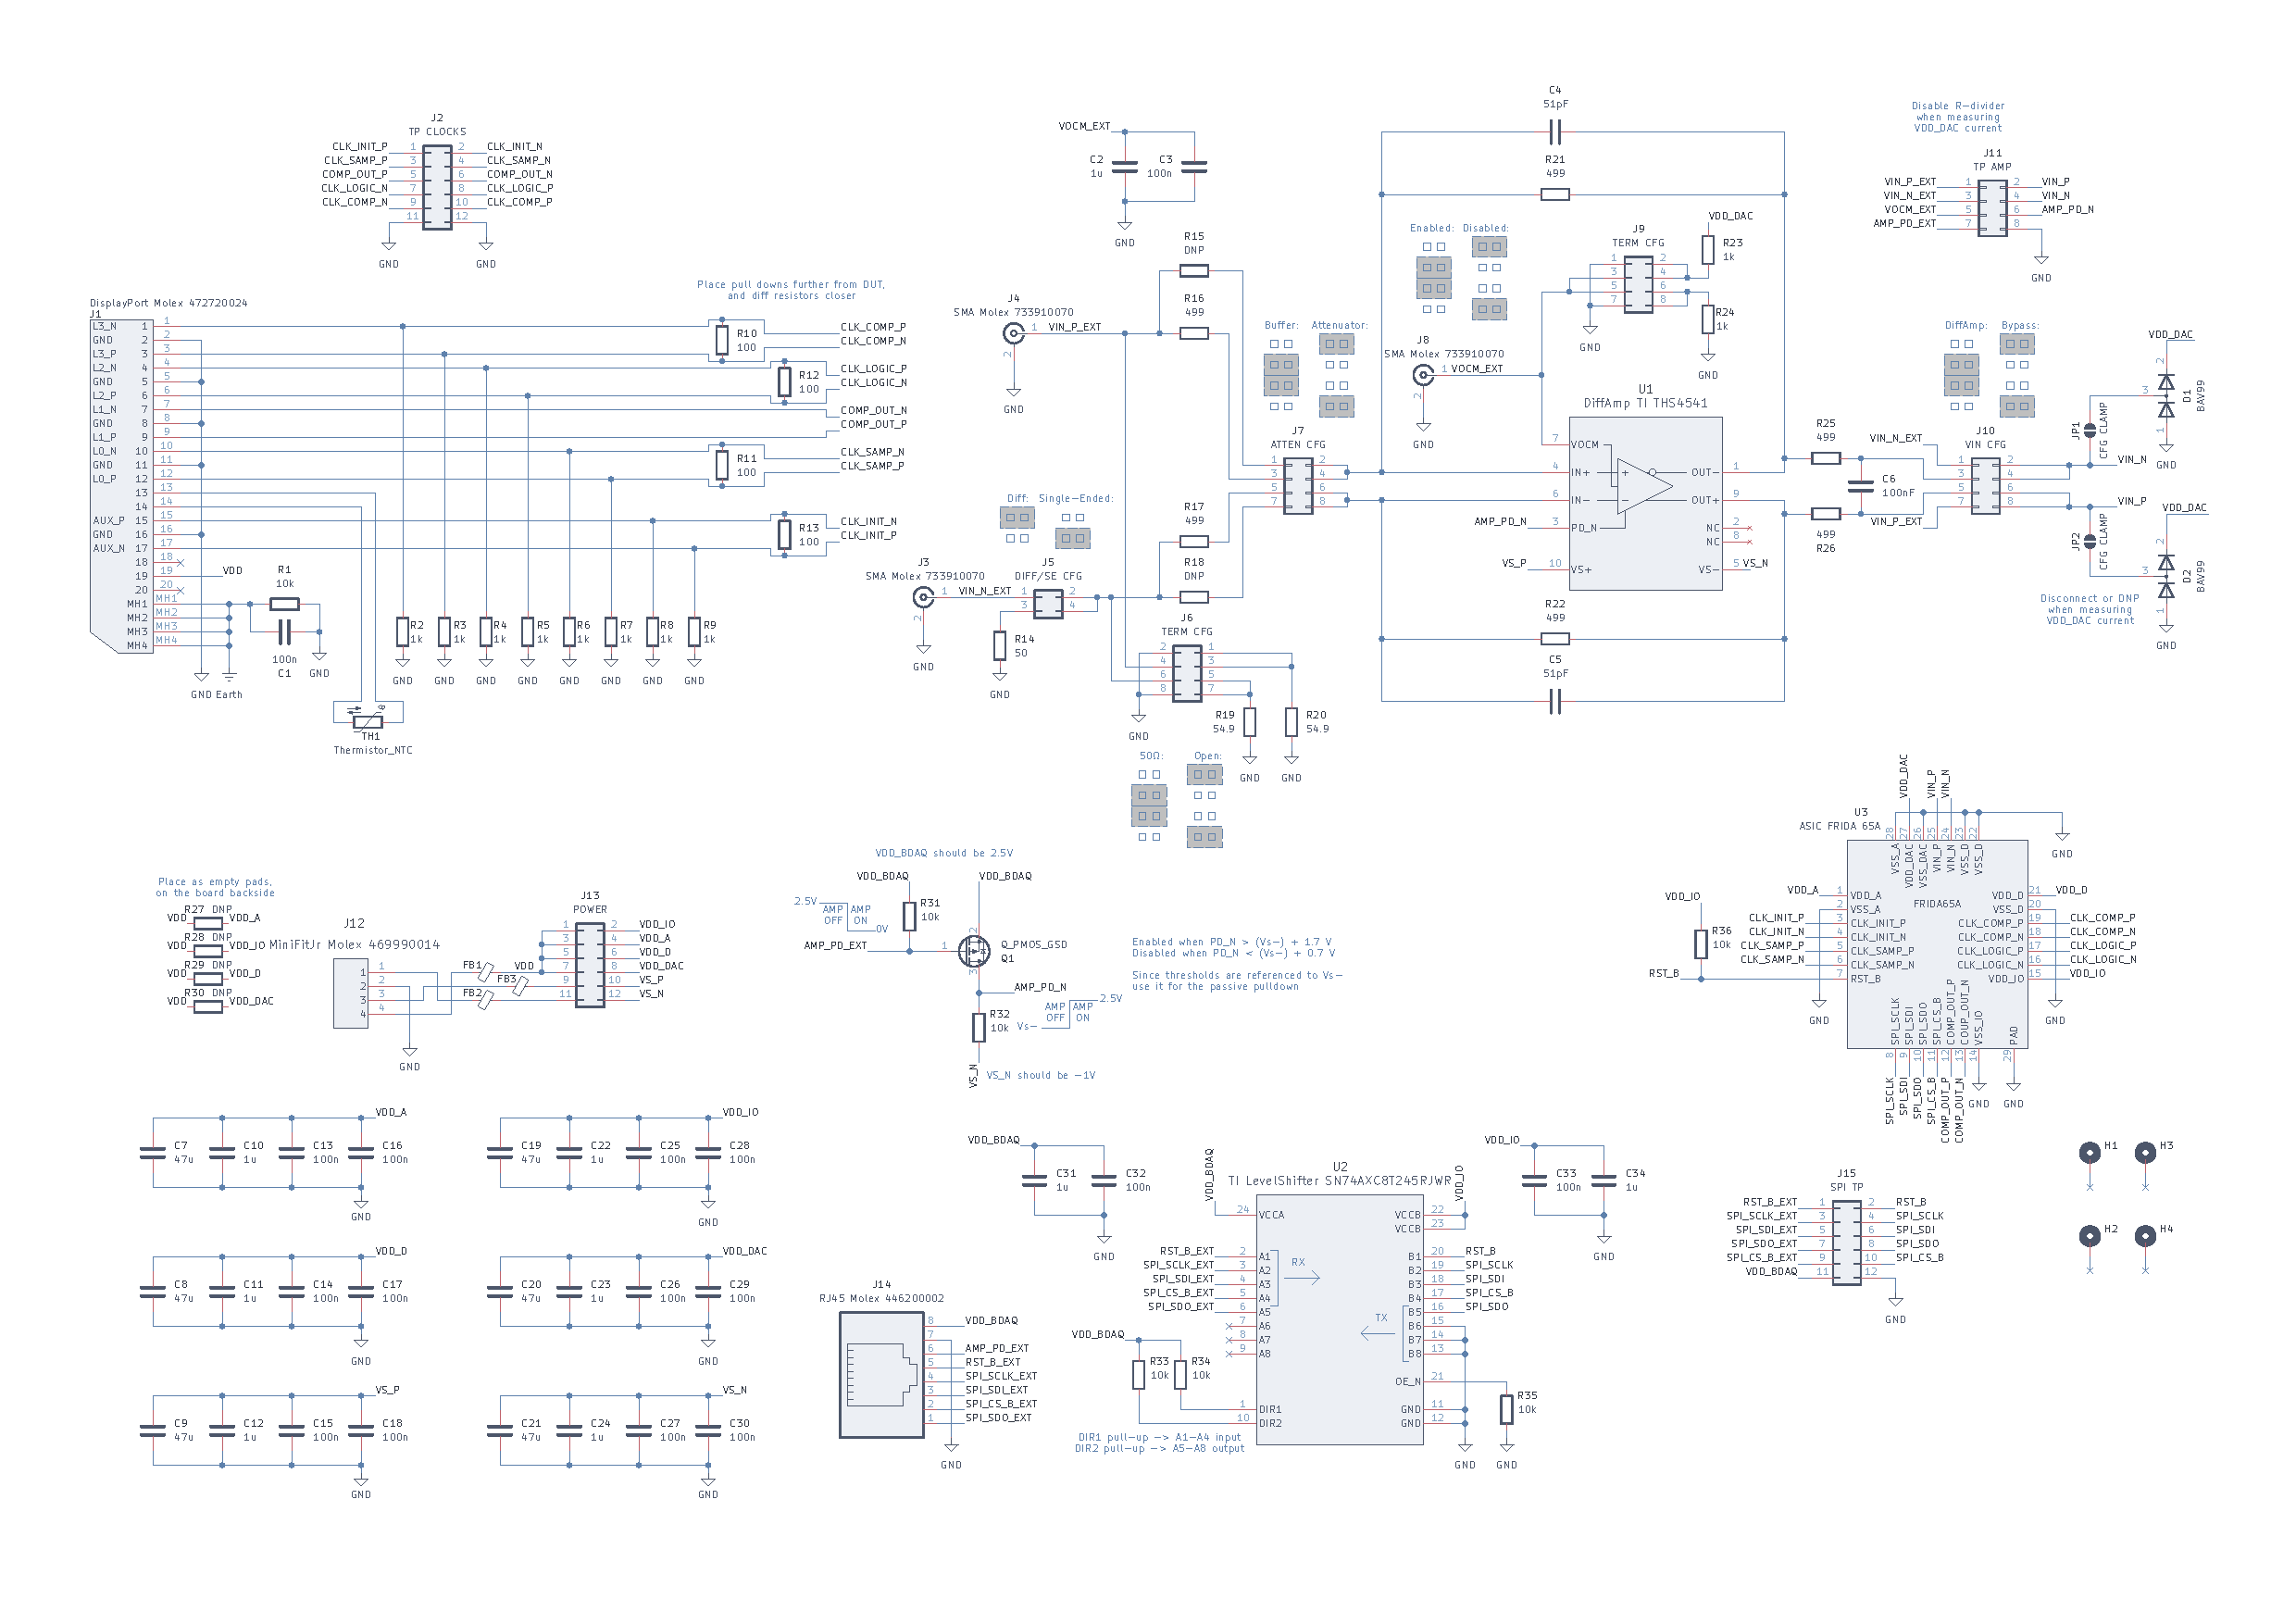
\includegraphics[width=420mm]{../images/interferer_hunt/frida65A_schematic.pdf}};
    % Probe locations: key, target point on the sheet, direction the arrow comes from.
    \schematic@arrow[45]{j11}{370.5}{34.5}{45}% J11 TP AMP pins 2/4: VIN_P/VIN_N, ADC side
    \schematic@arrow{j10}{352}{86}{120}% J10 VIN CFG pins 3/5: THS4541 outputs
    \schematic@arrow{j13}{104}{168}{60}% J13 POWER: all chip rails on VDD
    \schematic@arrow{j12}{63}{171}{120}% J12 MiniFit pins 1/3: amplifier +5 V / -1 V
    \schematic@arrow{r10}{132}{60}{60}% R10: COMP clock pair termination
    \schematic@arrow{j14}{161}{245}{150}% J14 RJ45 pin 8: VDD_BDAQ
    \schematic@arrow{j1}{38}{124}{-30}% J1 DisplayPort shield, GND Earth
    \schematic@arrow{u3}{327}{178}{150}% U3 ASIC: the output codes
    \schematic@arrow{loop}{345}{165}{60}% sniffer loop above the ASIC
    % Changed connections: key, box corners on the sheet.
    \schematic@box{j12}{46}{158}{80}{192}% J12 MiniFit: amplifier supply leads
  \end{tikzpicture}%
}
\makeatother

% A test's "where" frame: the title and the whole chip-card schematic, nearly
% full height, with one arrow at the probe location. #1 test title, #2 location
% key; the optional height is a fraction of the text height. The setup
% details are on the measurement plots that follow.
\newcommand{\testframe}[3][0.90]{%
  \begin{frame}[t]{#2}
    \vspace*{-1.2ex}%
    % Runs from under the title to the footer line; the zero-height box lets it
    % reach into the footline band without an overfull warning.
    \vbox to 0pt{\hbox to \linewidth{\hss\resizebox{!}{#1\textheight}{\schematicprobes{#3}}\hss}\vss}
  \end{frame}
}
% A frame for a test that probes nothing: the part whose connection changed is
% boxed instead. #1 test title, #2 location key.
\newcommand{\changeframe}[2]{%
  \begin{frame}[t]{#1}
    \vspace*{-1.2ex}%
    \vbox to 0pt{\hbox to \linewidth{\hss\resizebox{!}{0.90\textheight}{\schematicprobes[#2]{}}\hss}\vss}
  \end{frame}
}
% A result frame: one or two figures, nothing else.
\newcommand{\figframe}[2]{%
  \begin{frame}{#1}
    \centering
    \includegraphics[width=0.98\linewidth,height=0.80\textheight,keepaspectratio]{\figpath/#2}
  \end{frame}
}
\newcommand{\twofigframe}[3]{%
  \begin{frame}{#1}
    \centering
    \includegraphics[width=0.49\linewidth,height=0.80\textheight,keepaspectratio]{\figpath/#2}\hfill
    \includegraphics[width=0.49\linewidth,height=0.80\textheight,keepaspectratio]{\figpath/#3}
  \end{frame}
}

% Plain table cells: code sigma, and X/S/T timing-error counts below it.
\newcommand{\spreadvalue}[1]{#1}
\newcommand{\errorcount}[1]{#1}
\newcommand{\metric}[4]{\shortstack{\spreadvalue{#1}\\[-0.10em]\errorcount{#2}/\errorcount{#3}/\errorcount{#4}}}
% Measured cell: code sigma at 2, 6 and 10 MSPS; "stuck" marks four or fewer distinct codes.
\newcommand{\stuck}{stuck}
\newcommand{\rates}[3]{\shortstack{#1\\[-0.10em]#2\\[-0.10em]#3}}
\newcommand{\sequencepanel}[4]{%
  \begin{minipage}[t]{0.49\linewidth}
    \centering
    {\tiny COMP duty #3\,\%, LOGIC phase #4$^\circ$, LOGIC duty 50\,\%\par}
    \includegraphics[width=\linewidth,height=0.18\textheight,keepaspectratio,trim=5pt 8pt 5pt 5pt,clip]{../images/sequences/comp#1_logic#2.pdf}
  \end{minipage}%
}

\title{Hunting the 6--8 MHz ADC interferer}
\subtitle{From 9.6 to 10.25 ENOB at 2 MSPS by elimination}
\date{}

\begin{document}

\begin{frame}
  \titlepage
\end{frame}

\section[Overview]{Overview}

\begin{frame}{At 50\,\% COMP duty the ADC still shows 1.5--1.7 LSB: why?}
  \begin{columns}[c]
    \begin{column}{0.48\textwidth}
      \small
      \begin{itemize}
        \item At 2 MSPS every COMP duty cycle gives 1.5--1.7 LSB (ADC00: 1.68).
        \item Longer COMP high time (5/8--7/8) breaks down at 6--10 MSPS: wider spread, stuck codes.
        \item At 50\,\% duty it stays near 1.5--2 LSB from 2 to 10 MSPS, yet simulation expects 0.5--0.7 LSB.
        \item So two components: a \textbf{timing malfunction} that depends on duty and rate, and an \textbf{underlying random error} present at every setting.
        \item This deck hunts the second one.
      \end{itemize}
    \end{column}
    \begin{column}{0.50\textwidth}
      \centering
      {\footnotesize\setlength{\tabcolsep}{4pt}
      \begin{tabular}{@{}lccc@{}}
        \toprule
        COMP duty & 2 MSPS & 6 MSPS & 10 MSPS \\
        \midrule
        4/8 (50\,\%) & 1.47--1.68 & 1.43--2.02 & 1.71--3.25 \\
        5/8 & 1.48--1.68 & 1.87--3.13 & 2.55--3.95 \\
        6/8 & 1.44--1.69 & 1.89--4.12 & stuck--11.7 \\
        7/8 & 1.87--3.13 & stuck--14.9 & stuck--29.8 \\
        \bottomrule
      \end{tabular}
      \par\smallskip
      Code $\sigma$ in LSB over ADC00--03, 50 mV fixed input}
    \end{column}
  \end{columns}
\end{frame}

\begin{frame}{The seven ADC control sequences}
  \centering
  \sequencepanel{11110000}{00001111}{50}{180}\hfill\sequencepanel{11110000}{10000111}{50}{225}\par
  \sequencepanel{11111000}{10000111}{62.5}{225}\hfill\sequencepanel{11111000}{11000011}{62.5}{270}\par
  \sequencepanel{11111100}{11000011}{75}{270}\hfill\sequencepanel{11111100}{11100001}{75}{315}\par
  \sequencepanel{11111110}{11100001}{87.5}{315}\par
\end{frame}

\begin{frame}{Simulation: PEX code $\sigma$ and timing errors at 10 MSPS}
  \centering
  {\tiny\renewcommand{\arraystretch}{1.25}\setlength{\tabcolsep}{4.5pt}
  \begin{tabular}{@{}ccc*{7}{c}@{}}
    \toprule
    \shortstack{COMP\\duty (\%)} & \shortstack{LOGIC\\phase ($^\circ$)} & \shortstack{LOGIC\\duty (\%)} &
    \shortstack{FRIDA-1\\1 layer\\radix 1.7} & \shortstack{FRIDA-1\\1 layer\\radix 2.0} &
    \shortstack{FRIDA-1\\2 layers\\radix 1.7} & \shortstack{FRIDA-1\\2 layers\\radix 2.0} &
    \shortstack{FRIDA-2\\1 layer\\radix 1.7} & \shortstack{FRIDA-2\\2 layers\\radix 1.7} &
    \shortstack{FRIDA-2\\3 layers\\radix 1.7} \\
    \midrule
        50 & 180 & 50 & \metric{11.859}{40}{184}{197} & \metric{2.933}{3}{95}{16} & \metric{14.975}{32}{150}{253} & \metric{13.209}{0}{47}{136} & \metric{1.086}{45}{261}{90} & \metric{2.013}{15}{48}{249} & \metric{17.395}{18}{143}{197} \\
        50 & 225 & 50 & \metric{1.189}{61}{141}{1} & \metric{0.656}{21}{72}{0} & \metric{0.631}{43}{116}{0} & \metric{0.908}{19}{66}{0} & \metric{0.854}{47}{139}{0} & \metric{0.587}{44}{113}{0} & \metric{0.765}{26}{61}{0} \\
        62.5 & 225 & 50 & \metric{1.449}{4}{25}{49} & \metric{1.464}{1}{4}{20} & \metric{1.491}{3}{11}{24} & \metric{0.812}{5}{10}{21} & \metric{5.530}{0}{17}{35} & \metric{1.140}{2}{14}{27} & \metric{0.773}{1}{9}{17} \\
        62.5 & 270 & 50 & \metric{0.730}{4}{5}{0} & \metric{0.724}{1}{1}{0} & \metric{0.714}{2}{2}{0} & \metric{0.702}{0}{2}{0} & \metric{0.776}{4}{10}{0} & \metric{0.669}{1}{6}{0} & \metric{0.588}{2}{7}{0} \\
        75 & 270 & 50 & \metric{0.725}{0}{0}{0} & \metric{0.712}{0}{0}{0} & \metric{0.728}{0}{0}{1} & \metric{0.703}{0}{0}{0} & \metric{0.727}{0}{0}{1} & \metric{0.699}{1}{0}{1} & \metric{0.649}{0}{0}{1} \\
        75 & 315 & 50 & \metric{0.725}{0}{0}{0} & \metric{0.728}{0}{0}{0} & \metric{0.727}{0}{1}{0} & \metric{0.707}{0}{0}{0} & \metric{0.711}{0}{0}{0} & \metric{0.684}{0}{0}{0} & \metric{0.545}{0}{1}{0} \\
        87.5 & 315 & 50 & \metric{0.731}{0}{0}{0} & \metric{0.712}{0}{0}{0} & \metric{0.728}{0}{0}{0} & \metric{0.688}{0}{0}{0} & \metric{0.734}{0}{0}{1} & \metric{0.683}{0}{0}{0} & \metric{0.578}{0}{0}{0} \\
    \bottomrule
  \end{tabular}
  \par\smallskip
  Top: code $\sigma$ (LSB) over 100 conversions. Bottom: X/S/T timing errors of 1,700 decisions --
  X comparator below 0.3 V before COMP falls, S SR outputs wrong at LOGIC, T SR setup under 200 ps.\par}
\end{frame}

\begin{frame}{Silicon: code $\sigma$ at 2, 6 and 10 MSPS, amplifier supply unplugged}
  \centering
  {\tiny\renewcommand{\arraystretch}{1.35}\setlength{\tabcolsep}{3.2pt}
  \begin{tabular}{@{}ccc|ccc|ccc|ccc|ccc@{}}
    \toprule
    & & & \multicolumn{3}{c|}{\shortstack{ADC00 FRIDA-1\\1 layer, radix 1.7}} & \multicolumn{3}{c|}{\shortstack{ADC01 FRIDA-1\\1 layer, radix 2.0}}
    & \multicolumn{3}{c|}{\shortstack{ADC02 FRIDA-1\\2 layers, radix 1.7}} & \multicolumn{3}{c}{\shortstack{ADC03 FRIDA-1\\2 layers, radix 2.0}} \\
    \shortstack{COMP\\duty (\%)} & \shortstack{LOGIC\\phase ($^\circ$)} & \shortstack{LOGIC\\duty (\%)} &
    2 & 6 & 10 & 2 & 6 & 10 & 2 & 6 & 10 & 2 & 6 & 10 \\
    \midrule
    50 & 180 & 50 & \spreadvalue{0.99} & \spreadvalue{1.20} & \spreadvalue{1.38} & \spreadvalue{0.94} & \spreadvalue{1.28} & \spreadvalue{33.26} & \spreadvalue{0.88} & \spreadvalue{0.95} & \spreadvalue{8.89} & \spreadvalue{1.02} & \spreadvalue{1.03} & \spreadvalue{1.48} \\
    50 & 225 & 50 & \spreadvalue{0.98} & \spreadvalue{1.11} & \spreadvalue{1.40} & \spreadvalue{0.94} & \spreadvalue{1.27} & \spreadvalue{2.87} & \spreadvalue{0.88} & \spreadvalue{0.87} & \spreadvalue{1.23} & \spreadvalue{1.03} & \spreadvalue{0.98} & \spreadvalue{1.46} \\
    62.5 & 225 & 50 & \spreadvalue{0.99} & \spreadvalue{1.73} & \spreadvalue{3.19} & \spreadvalue{0.94} & \spreadvalue{2.90} & \spreadvalue{32.83} & \spreadvalue{0.88} & \spreadvalue{1.38} & \spreadvalue{6.97} & \spreadvalue{1.03} & \spreadvalue{1.95} & \spreadvalue{2.71} \\
    62.5 & 270 & 50 & \spreadvalue{0.99} & \spreadvalue{1.73} & \spreadvalue{3.17} & \spreadvalue{0.94} & \spreadvalue{2.92} & \spreadvalue{1.90} & \spreadvalue{0.88} & \spreadvalue{1.39} & \spreadvalue{3.15} & \spreadvalue{1.04} & \spreadvalue{1.90} & \spreadvalue{2.72} \\
    75 & 270 & 50 & \spreadvalue{1.03} & \spreadvalue{3.85} & \spreadvalue{11.54} & \spreadvalue{0.95} & \spreadvalue{2.09} & \stuck & \spreadvalue{0.90} & \spreadvalue{3.72} & \spreadvalue{4.27} & \spreadvalue{0.97} & \spreadvalue{1.11} & \spreadvalue{3.49} \\
    75 & 315 & 50 & \spreadvalue{1.02} & \spreadvalue{3.91} & \spreadvalue{11.61} & \spreadvalue{0.96} & \spreadvalue{2.11} & \stuck & \spreadvalue{0.91} & \spreadvalue{3.70} & \spreadvalue{4.24} & \spreadvalue{0.98} & \spreadvalue{1.04} & \spreadvalue{3.40} \\
    87.5 & 315 & 50 & \spreadvalue{1.78} & \stuck & \spreadvalue{6.56} & \spreadvalue{2.95} & \stuck & \spreadvalue{1.19} & \spreadvalue{1.40} & \spreadvalue{13.55} & \stuck & \spreadvalue{1.95} & \stuck & \spreadvalue{24.55} \\
    \bottomrule
  \end{tabular}
  \par\smallskip
  Code $\sigma$ (LSB) per conversion rate (MSPS), 100,000 conversions each (test \#12).
  stuck: under 0.3 LSB from four or fewer codes.\par}
\end{frame}

\begin{frame}{Expressions used throughout}
  \footnotesize
  \begin{columns}[T]
    \begin{column}{0.5\textwidth}
      \begin{align*}
        V_\mathrm{LSB} &= \frac{V_\mathrm{ref}}{2^N} = \frac{1.2\,\mathrm{V}}{4096} \approx 293\,\mu\mathrm{V} \\
        \mathrm{ENOB} &= N - \log_2\frac{\sigma_\mathrm{code}}{1/\sqrt{12}\ \mathrm{LSB}} \\
        v_\mathrm{rms}^2 &= \int_{f_1}^{f_2} S_v(f)\,df, \quad \sqrt{S_v}\ \text{in V}/\sqrt{\mathrm{Hz}} \\
        v_\mathrm{rms} &= e_n\sqrt{B} \quad \text{(flat density only)}
      \end{align*}
    \end{column}
    \begin{column}{0.5\textwidth}
      \begin{align*}
        \sigma^2 &= \sigma_\mathrm{interferer}^2 + \sigma_\mathrm{broadband}^2 \\
        f_a &= \left|\big((f + f_s/2) \bmod f_s\big) - f_s/2\right| \\
        v_d &= v_p - v_n, \qquad v_{cm} = \tfrac{1}{2}(v_p + v_n) \\
        V_\mathrm{line} &\approx \sqrt{S_v(f_0)\,\mathrm{ENBW}}, \quad \mathrm{ENBW}_\mathrm{Hann} = 1.5\,\Delta f
      \end{align*}
    \end{column}
  \end{columns}
\end{frame}

\section[Input]{Input chain}

\figframe{Test \#1: scope floor, shorted 1X probes, to know the smallest noise we can see}{step1_floor_probes_spectrum.pdf}

\figframe{Test \#2: divider supply, FPGA on the shared 5 V, to see if the input source is clean}{step2_supply_div_shared.pdf}

\testframe{Test \#3: VIN\_P/VIN\_N at J11, ADC idle, to check the input reaching the ADC}{j11}

\figframe{Test \#3a: VIN\_P/VIN\_N at J11, FPGA on the shared 5 V, to see what it adds}{step3_shared_supply.pdf}

\figframe{Test \#3b: VIN\_P/VIN\_N at J11, FPGA on its own E3634A, to confirm a quiet input}{step3_own_supply.pdf}

\section[ADC]{ADC codes}

\figframe{Test \#4: no probe; ADC codes as a waveform, to split lines from broadband}{code_noise_20261008.pdf}

\twofigframe{Test \#4: aliases at three rates, to find the interferer's true frequency}{code_spectra_20261008.pdf}{interferer_20261008.pdf}

\section[Probing]{Probing}

\testframe{Test \#5: VDD at J13, ADC converting, to see if the chip supply carries it}{j13}

\figframe{VDD carries nothing at the interferer frequency}{hunt_vdd_a_spectrum.pdf}

\testframe{Test \#6: DP shield against card ground, ADC converting, to find a ground loop}{j1}

\figframe{No ground difference at the interferer frequency}{hunt_gnd_bdaq_spectrum.pdf}

\testframe{Test \#7: VDD\_BDAQ at J14 pin 8, ADC converting, to check the FPGA I/O supply}{j14}

\figframe{VDD\_BDAQ is clean too}{hunt_vdd_bdaq_spectrum.pdf}

\testframe{Test \#8: VIN\_P/VIN\_N at J11, ADC converting, to see if it is on the input}{j11}

\figframe{The ADC inputs stay quiet while it converts}{hunt_vin_diff.pdf}

\testframe{Test \#9: COMP clock pair at R10, sequencer idle, to see if the clocks carry it}{r10}

\figframe{The idle COMP pair is quiet}{hunt_clk_comp_diff.pdf}

\testframe{Test \#10: loops at ASIC, E3634A, FPGA, ADC converting, to find a radiator}{loop}

\twofigframe{Sniffer loops find the FPGA module's switchers, not the interferer}{sniff_e3634a_fpga_spectrum.pdf}{sniff_asic_fpga_spectrum.pdf}

\section[A/B]{Elimination}

\testframe{Test \#11: diff-amp outputs at J10, ADC converting, to see if it oscillates}{j10}

\figframe{The amplifier outputs are clean too}{step6_amp_out_spectrum.pdf}

\changeframe{Test \#12: no probe; amp supply unplugged at J12, to see if it leaves too}{j12}

\figframe{Without the amplifier supply, the interferer is gone}{code_noise_A.pdf}

\changeframe{Test \#13: no probe; amp supply on at J12, AMP\_EN on, to see if it returns}{j12}

\figframe{With the supply back, so is the interferer}{code_noise_B.pdf}

\changeframe{Test \#14: no probe; amp supply on, AMP\_EN off, to rule out oscillation}{j12}

\figframe{A powered-down amplifier still lets it in}{code_noise_C.pdf}

\changeframe{Test \#15: no probe; amp leads in, supply turned down, to rule out a ground loop}{j12}

\figframe{Leads in but no supply voltage: clean, so no ground loop}{code_noise_D.pdf}

\figframe{All runs side by side}{amp_supply_code_spectra.pdf}

\section[Next]{Next steps}

\begin{frame}{Next steps}
  \begin{itemize}
    \item Split the TOE 8733 rails: V+ at +5 V with V$-$ at 0 V, then V+ at its minimum with V$-$ at $-$1 V.
    \item Power the amplifier from a second supply; fix by filtering at J12 or a quieter source.
    \item Find what back-feeds VS\_P to 0.8 V when its supply is turned down.
    \item The fixed 2856-kHz line at 10 MSPS unfolds to 7.143 MHz (200 MHz/28?).
    \item Keep the amplifier unpowered in divider mode (\texttt{-k amp\_off} in \texttt{test\_noise.py}).
    \item Decode the clean run with calibrated weights to separate DNL from noise.
    \item Revisit the 6/8--7/8 reset limits at high rate.
  \end{itemize}
\end{frame}

\section[Index]{Index}

\begin{frame}{Index of tests}
  \centering
  {\scriptsize
  \begin{tabular}{@{}rll@{}}
    \toprule
    Test & Probed & Condition \\
    \midrule
    \#1 & Scope floor, shorted 1X probes & --- \\
    \#2 & Divider supply & FPGA on the shared 5 V \\
    \#3a & VIN\_P/VIN\_N at J11 & ADC idle; FPGA on the shared 5 V \\
    \#3b & VIN\_P/VIN\_N at J11 & ADC idle; FPGA on its own E3634A \\
    \#4 & No probe: ADC output codes & 2, 6 and 10 MSPS, seven sequences \\
    \#5 & VDD at J13 & ADC converting \\
    \#6 & DP shield against card ground & ADC converting \\
    \#7 & VDD\_BDAQ at J14 pin 8 & ADC converting \\
    \#8 & VIN\_P/VIN\_N at J11 & ADC converting \\
    \#9 & COMP clock pair at R10 & sequencer idle \\
    \#10 & Loops at the ASIC, E3634A and FPGA & ADC converting \\
    \#11 & Diff-amp outputs at J10 & ADC converting \\
    \#12 & No probe: ADC output codes & amp supply unplugged at J12 \\
    \#13 & No probe: ADC output codes & amp supply on, AMP\_EN on \\
    \#14 & No probe: ADC output codes & amp supply on, AMP\_EN off \\
    \#15 & No probe: ADC output codes & amp leads in, supply turned down \\
    \bottomrule
  \end{tabular}
  }
\end{frame}

\end{document}
